
% Other exposed or explicit datapath architectures and their corresponding compilers.

% Other pure SIMD architectures, GPU and its difference if i know this and can tell it.

% Liu's work on compiler design, and what it lacks, proper support for 5-stage configuration, explicit bypass conf. 

%Old rel. work
There is related work for compilers that target SIMD architectures, in particular, a compiler has been developed, referred to as legacy compiler. Furthermore, there is related work in building an LLVM backend, and compiling with explicit datapaths has been an active research topic for other architectures.
% scrap
%The related work is introduced in this part, including the legacy compiler, building the LLVM back-end for SIMD architecture, explicit datapaths in other architecture and some scheduling and register allocation algorithms applied in other compilers.

%\section{Building an LLVM back-end}
%Our backend is derived from tricore tutorial on creating a new backend for the LLVM compiler framework \cite{tricore}. Furthermore, based on that work, an LLVM backend for SIMD architecture without explicit bypassing has been developed \cite{liu_zhenyuan}. However, the current compiler generates code with implicit bypassing. We, therefore, need to extend this to efficiently generate code for explicit bypassing as well. Therefore, our work will be an extension to previously noted work.

\subsection{Other Exposed/Explicit Datapath Architectures}\label{sec:other_explicit_datapaths}
Compiling with explicit datapaths has been an active topic of research. Several architectures that face similar challenges have been investigated. 

%Johan janssen & ... TTA work
%Other exposed datapaths

\subsubsection{Transport Triggered Architectures}\label{sec:tta}
One of the main works that was investigated is the  \emph{Transport Triggered Architecture} (TTA) which has been developed in the MOVE project \cite{tta_codegen}. For TTA architectures, instructions consist of transports that specify the datapath. The difference between TTAs and traditional operation triggered architectures is that TTA are transport driven, hence its name. 

Figure \ref{fig:tta} illustrates how function units and register files are connected to an interconnect network which are programmed by instructions. Programming a TTA consists of moving operands to the input registers of a FU.

\begin{figure}[b!]
\centering
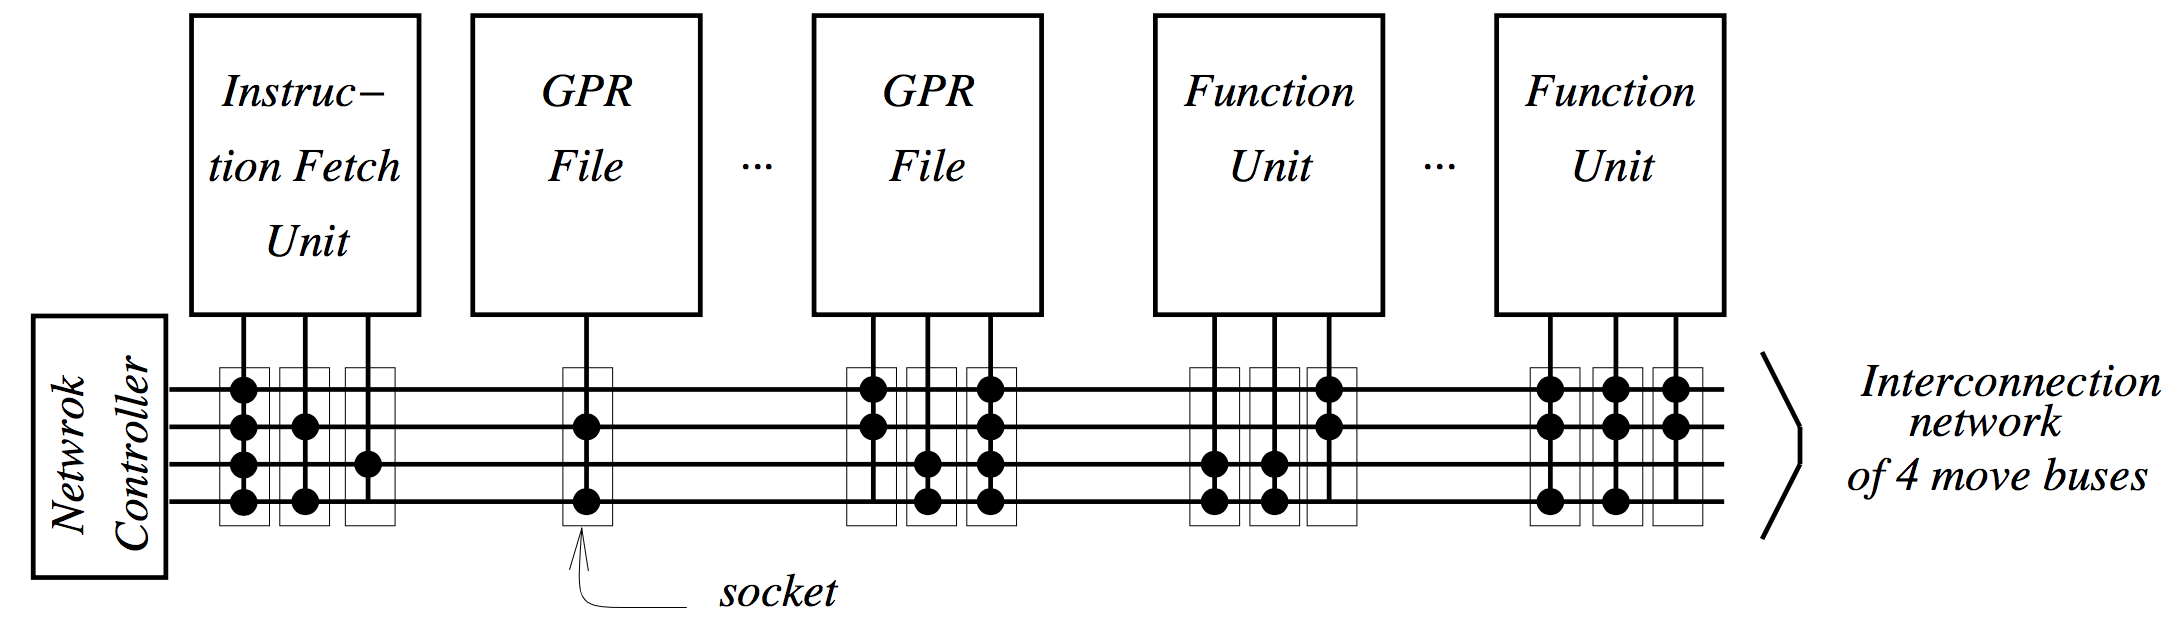
\includegraphics[width=.8\textwidth]{figures/tta_structure}
\caption{General structure of a TTA with interconnect network driven by data transports.}
\label{fig:tta}
\end{figure}

%\lstset{style=customasm}
\begin{lstlisting}
add r1, r2, r3  # define r1 with r1 = r2 + r3
sub r4, r2, 6   # define r4 with r4 = r2 - 6
sw  r4, r1, 0   # store result at address r1
\end{lstlisting}

First step is to translate each $n$-operand $m$-result operation into $n+m$ moves (so called $n$ \emph{operand moves} and $m$ \emph{result moves}). \texttt{O1} and \texttt{O2} are input ports of the FU and \texttt{R} indicates the output (result) of a FU.
%Insert more text explaining both fragments above and below this paragraph.

\begin{lstlisting}
r2 -> O1add ; r3 -> O2add ; Radd -> r1
r2 -> O1sub ; r6 -> O2sub ; Rsub -> r4
r1 -> O1sw  ; r4 -> O2sw
\end{lstlisting}

Let us assume that there are two FUs named \texttt{alu1} and \texttt{alu2} for ALU operations, and one FU named \texttt{ls} for load-store operations. The suffixes `\texttt{alu1}', `\texttt{alu2}', and `\texttt{ls}' indicate the FU on which the operation is executed.
If the above fragment would be scheduled such that the distance between the final operand and a corresponding result move should be at least the latency of the FU. Then the following (TTA assembly) code may be obtained:

\begin{lstlisting}
r2 -> O1add.alu1 ; r3 -> O2add.alu1 ; r2 -> O1sub.alu2 ; r6 -> O2sub.alu2
Radd.alu1 -> r1  ; Rsub.alu2 -> r4
r1 -> O1sw.ls    ; r4 -> O2sw.ls
\end{lstlisting}


\textbf{Bypassing:} The outputs of the add and subtract operations can be directly moved to the load-store unit. This reduces the schedule by one cycle, however, the number of moves does not change.

\begin{lstlisting}
r2 -> O1add.alu1; r3 -> O2add.alu1; r2 -> O1sub.alu2    ; r6 -> O2sub.alu2
Radd.alu1 -> r1 ; Rsub.alu2 -> r4 ; Radd.alu1 -> O1sw.ls; Rsub.alu2 -> O2sw.ls
\end{lstlisting}

\textbf{Dead result move elimination:} Next it may occur that the values in \texttt{r1} and \texttt{r2} are not live anymore because they are used only once. In that case corresponding moves can be skipped. This gives the following schedule:

\begin{lstlisting}
r2 -> O1add.alu1 ; r3 -> O2add.alu1 ; r2 -> O1sub.alu2 ; r6 -> O2sub.alu2 
Radd.alu1 -> O1st.ls ; Rsub.alu2 -> O2st.ls
\end{lstlisting}

The optimizations that is discussed here for TTA also apply on a wide SIMD architecture, which is discussed in Section \ref{sec:datapaths}. However, their approach can not be used because the SIMD architecture is an operation triggered architecture, data transports are a given. More information on explicit bypassing for TTAs can be found in the work of Hoogerbrugge et. al. \cite{tta, tta_codegen}.

%TODO read chapter 7 and cite to it, add words about TTA compiler. Then can be used yes/no

\begin{figure}[b!]
\centering
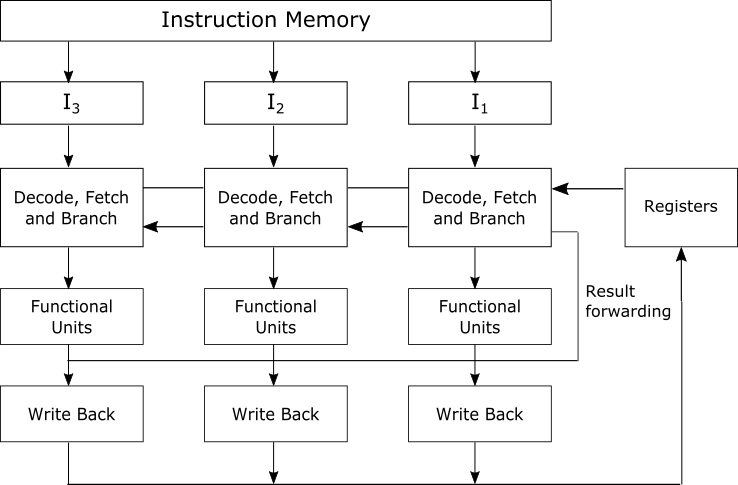
\includegraphics[width=.65\textwidth]{figures/vliw_forwarding}
\caption{Block diagram of VLIW architecture with bypassing.}
\label{fig:vliw}
\end{figure}

\subsubsection{Very Long Instruction Word Architectures}
The \emph{Very Long Instruction Word} (VLIW) architecture is designed to optimize \emph{Instruction Level Parallelism} (ILP) by executing multiple instructions in parallel.
Although RISC architectures take advantage of temporal parallelism by using hardware pipelining (explained in Chapter \ref{sec:datapaths}), VLIW architectures take advantage of spacial parallelism by using multiple functional units to execute several operations concurrently. 

Figure \ref{fig:vliw} shows a generic block diagram of a VLIW machine that has multiple instruction issues (three in this example), and each issue has its own decode stage and functional units. The figure also illustrates how the bypass network connects the outputs of the FUs back to the ID stage, allowing results to be forwarded. For VLIW architectures, the complexity of the bypass network grows linearly with the size of the instruction word. Furthermore, traditionally the register file requires $n$ write and $2n$ read ports, where $n$ is the length of the instruction word. This may require a more hungry register file as the power efficiency degrades when increasing the number of ports on the register file \cite{compiler_driven_power_opt}. However, this requirement can be relaxed by clustering, where each cluster may have a dedicated register file, which is often done in modern VLIW architectures.\\

A reconfigurable VLIW architecture is developed in the $\rho$-VEX project at the University of Technology in Delft \cite{p-vex}. This architecture also considers explicit bypassing and other configurable design options, e.g. configurable issue-width, functional units and bit-width of the data.

However, their implementation can not be used because (i) they are using a gcc based compiler instead of a LLVM based compiler and (ii) not a lot of implementation details have been given in their paper.



%\subsubsection{ReMove}
%Another architecture that exploits explicit datapath architectures is the ReMove architecture \cite{remove}. That work focusses on scheduling for partially connected architectures with explicit datapaths. The ReMove architecture is similar to a VLIW, having multiple FUs, however here they have an interconnect network that connects the FUs to the RF. The scheduling algorithm used in this work can not be used in our work, because similar to the legacy compiler for SIMD, this project has a custom backend, which can not be reused for LLVM. However, the basic principles of the scheduling algorithms proposed in this work are still valid and may be reused for our work.

%\section{Scheduling and Register Allocation}
%First of all, from the existing scheduling algorithms, Swing Modulo Scheduling (SMS) seems to be a suitable scheduling approach. It is a heuristic approach that is able to deal efficiently with software pipelining. Furthermore, it is known for its outstanding performance and low computational cost. The generated schedules are near optimal in terms of initiation interval and register requirements \cite{swingmodulo_paper, swingmodulo_thesis}. We consider this a candidate scheduler to use.

%Furthermore, the following literature discusses register allocation for SSA-based programs that solves coloring problem optimally in quadratic-time optimal by decoupling coloring, spilling and coalescing \cite{ra}. This technique may allow us to implement a custom register allocator that solves the problem in polynomial time.

%Finally, there is another project, called Unison. They solve scheduling and register allocation and other code generation tasks by translating them into combinatorial problems and solve them together with constraint programming \cite{unison}. We consider this a candidate constraint solver to use because it can be easily integrated with LLVM.

\subsection{Legacy compiler}\label{sec:legacy_comp}
S. Dongrui et al. proposed this processor architecture \cite{simd} while attaining his PhD \cite{dongrui}. The target wide SIMD architecture was design during that time and the compiler that was developed then has many issues. To start, the compiler has a LLVM frontend and a mostly in C++ implemented backend which is not according to LLVM standard. Therefore, it requires a frontend based on an old version of LLVM and since its front-end evolves over time, it is preferable to be able to update this to the newest version. \\

With C code applications as input language, the compiler can only compile to non-vectorized (CP only) instructions. To generate vectorized code an effort had been made to take OpenCL code as input language \cite{dongrio2}. However, only a subset of OpenCL is supported. Moreover, compilation does often generate incorrect code, or none at all. \\


In his work he shows that the register file is one of the most frequently used, and most power-hungry components in a processor. Therefore, he introduced an explicit datapath to further improve energy efficiency on this extremely energy efficient processor architecture. Moreover, efficient code generation for such architecture is key to achieve high energy efficiency for the whole processor. For this reason, the efficiency of the generated code is improved by standardizing the compiler to a frequently used framework. Namely, by standardizing to LLVM. This way we may benefit from developments in the field of compilers and from improvements made to the LLVM framework.
%A compiler had already been developed during the design phase of the target wide SIMD architecture \cite{dongrui}. That compiler has an assembler that can translate from assembly to object code and the compiler can translate C code to scalar only- and OpenCL to vectorized assembly code or object code. That compiler consists of a LLVM front-end and the back-end is developed in C++, but not within the LLVM framework.

%The legacy compiler was developed by the ES group in 2003. We will use the SIMD architecture as it was designed during that time . The legacy compiler has a custom backend for the SIMD architecture that can generate code for explicit datapaths \cite{dongrio1}, but it can only compile C code to non-vectorized instructions or a small subset of hand-touched OpenCL code that also requires manual insertion of custom pragmas to compile for vectorized code \cite{dongrio2}. Our goal is to overcome certain limitations and improve the compilers maintainability.
 

%Dongrio's simd work 

\subsection{Basic Compiler Design}\label{sec:basic_compiler_design}
This section explains an initial design of a SIMD back-end designed within LLVM developed by L. Zhenyuan \cite{liu_zhenyuan}. He started to build a back-end in LLVM for the same purpose, but with a different goal, namely how to generate efficient vectorized code within LLVM. In order to support vector instructions, LLVM's auto-vectorizer has been used and intermediate code optimization passes have been implemented to generate SIMD specific intrinsics, that are, in turn, transformed to vector instructions and shuffle operations. 

His work gives a basic design for this back-end that targets a wide SIMD architecture. The compiler that he developed is taken as a starting point, and is maintained, improved and extended which is discussed in later sections. When building a back-end in LLVM, first the instructions and registers have to be defined. Then illegal operations and types can be converted to legal ones. Then during instruction selection, LLVM knows how to match DAG nodes to known instructions. The supported instructions and registers for this architecture are defined first. To support some special features of this architecture, custom passes are added to this back-end, which will be described in detail, see Chapter \ref{sec:code_generation}, where our contributions to this work are discussed. Furthermore, an assembler and a linker have been implemented as separate projects, which will briefly be discussed here as well.

\subsubsection{Supported Instructions}
All the instructions which have been defined in this compiler are listed in this part, with the corresponding brief explanations. The details of ISA can be found in Appendix \ref{appendix:A}.
\begin{itemize}
	\item \textbf{Arithmetic and Logic Instructions:} \texttt{add}, \texttt{addi}, \texttt{sub}, \texttt{muli}, \texttt{mulu}, \texttt{mului}, \texttt{or}, \texttt{ori}, \texttt{and}, \texttt{andi}, \texttt{xor}, \texttt{xori}, \texttt{sll}, \texttt{slli}, \texttt{sra}, \texttt{srai}, \texttt{srl} and \texttt{srli}.\\
The instruction with suffix "I" is used to handle immediate value operand, which is referred to as I-type instructions. The suffix "U" means it is used for unsigned values. For others, the two input operands are both registers, which are commonly referred to as R-type instructions.
	\item \textbf{Flag Set Instructions:} \texttt{sfeq}, \texttt{sfne}, \texttt{sfles}, \texttt{sflts}, \texttt{sfges}, \texttt{sfgts}, \texttt{sfleu}, \texttt{sfltu}, \texttt{sfgeu} and \texttt{sfgtu}.\\
The flag set instructions are used for comparison. If it is true, the flag register is set. The suffix "S" represents a signed value, while the suffix "U" represents an unsigned value.
	\item \textbf{Conditional Move:} \texttt{cmov}.\\ This is usually used with flag set instructions. If the flag is set, the value in the input operand is moved to the output operand.
	\item \textbf{Immediate Extension:} \texttt{simm} and \texttt{zimm}.\\ These two instructions are used to extend the immediate value from 8 bits to 26 bits. The maximum immediate value could be $2^{26}-1$, instead of $2^8-1$. The details of these two instructions will be discussed in Section \ref{sec:immediate_ext}. In addition, a larger immediate value requires a sequence of instructions to be executed.
	\item \textbf{Conditional Branch:} \texttt{bf} and \texttt{bnf}.\\ These two instructions also work with flag set instructions. By using the branch in- structions, the program can branch to the target address if the flag is set (with BF) or not set (with BNF).
	\item \textbf{Jump Instructions:} \texttt{j}, \texttt{jr}, \texttt{jal} and \texttt{jalr}.\\ The difference with the conditional branch instructions is that the jump does not need to check the flag register, which is normally used during function call and return.
\end{itemize}

\subsubsection{Register Configuration}
There are two main register classes. Although each PE has its own register file in our architecture, it is not necessary to define a specific register class for every PE register file. One reason is the size of the PE array is configurable and the number of the vector register classes cannot be dynamic. Another reason is, the vector array actually is a single issue slot, which executes the same instruction for all PEs. It is sufficient to define one register class for the entire PE array. Each vector register defined in the back-end represents a line of registers in the PE array.

\begin{table}[t]
\caption{Registers configuration.}
\begin{center}
\begin{tabular}{@{}l l l@{}}
\toprule
\textbf{Scalar Register} & \textbf{Vector Register} & \textbf{Purpose} \\ \hline
\texttt{r0} & \texttt{v0} & Constant value zero \\
N/A & \texttt{v1} & Constant PE index \\
\texttt{r3}$\sim$\texttt{r4}  & \texttt{v3}$\sim$\texttt{v4} & Return registers \\
\texttt{r5}$\sim$\emph{r8} & \texttt{v5}$\sim$\texttt{v8} & Argument passing registers \\
\texttt{r9} & N/A & Link register \\ 
\texttt{r10} & N/A & Frame pointer \\
\texttt{r11} & \texttt{v11} & Stack pointer \\
\texttt{r1}, \texttt{r2} and \texttt{r12}$\sim$\texttt{r31} & \texttt{v2}, \texttt{v9}$\sim$\texttt{v10} and \texttt{v12}$\sim$\texttt{v31} & General purpose registers \\
\bottomrule
\end{tabular}
\end{center}
\label{table:register_conf}
\end{table}%
%TODO: add text that goes by this, and optionally change lists in tables.

Table \ref{table:register_conf} shows the register configurations of both CP and PE-Array.
Both \texttt{r0} and \texttt{v0} are connected to ground and contain constant value zero. \texttt{v1} is a special register, which contains the index of local PE. Note that, there are two stack pointers, \texttt{r11} and \texttt{v11}. As mentioned before, considering there are two separated data memory, a double frame stack is needed for the CP and PE-Array to access their memories directly and reduce the expensive data communication. Therefore, two stack pointers are defined to point to the top of scalar and vector frame stacks respectively. The details of separate frame stacks is not described here, but can be found in L. Zhenyuans thesis \cite[Chapter~4]{liu_zhenyuan}.

\subsubsection{Vectorizer}
 Support for LLVM's Auto-Vectorizer has been developed by L. Zhenyuan. He added support for this to our back-end during his time \cite[Chapter~5]{liu_zhenyuan}. He defined a couple of patterns to match and IR level transformations that transform loops to vector instructions and shuffle operations. Furthermore, he added a cost function to decide whether to vectorize a given loop automatically. However, sometimes the auto-vectorizer fails to vectorize a simple loop. In those cases, pragmas are manually inserted directly before a loop in the C code. Clang uses these pragmas for making decisions on whether or not to vectorize a given loop. In the end, this may give better results, as will be shown in Chapter \ref{chapter:evaluation}.
 
 Supported vector types are:
 \texttt{v1i32}, \texttt{v2i32}, \texttt{v4i32}, \texttt{v8i32}, \texttt{v16i32}, \texttt{v32i32}, \texttt{v64i32}, \texttt{v128i32}, \texttt{v256i32}, \texttt{v512i32}, \texttt{v1024i32} and \texttt{v2048i32}.\\
	The actual legal vector type should be equal to or smaller than the \texttt{PENum}. \texttt{PENum} is a variable defined in the back-end, which can be configured using \texttt{pe-num} flag. The default value is 8, in which case the legal vector type can only be \texttt{v1i32}, \texttt{v2i32}, \texttt{v4i32} and \texttt{v8i32}.

\subsubsection{Linker and Assembler}
An assembler has been implemented that can parse assembly code and translate it into binary code. Furthermore, a linker has been developed which takes one or more binary files and combines them into a single executable file. These have been developed as separate projects and within the LLVM framework. Unfortunately, the linker still has some problems that need to be resolved before it can be used. %TODO go deeper into limitations of the lld linker
Therefore, a custom linker is chosen instead of the standard linker supplied by LLVM. We would benefit from using LLVM's linker because the custom linker can work only on a single file. Unfortunately, this linker can not be used yet because it is a work in progress.%work in progress

%TODO: add bypassing, auto and expl, (from slides)

